% Analyse des résultats de l'expérience 1 - Llama-3.1-8B-Instruct
% Source : results/experiment1/full32_all (306 280 essais)
% Compilation : pdflatex experiment1-llama-analyse.tex (deux passes)
\documentclass[11pt,a4paper]{article}

\usepackage[utf8]{inputenc}
\usepackage[T1]{fontenc}
\usepackage[french]{babel}
\usepackage{lmodern}
\usepackage[margin=2.4cm]{geometry}
\usepackage{amsmath,amssymb}
\usepackage{booktabs}
\usepackage{graphicx}
\usepackage{caption}
\usepackage{siunitx}
\usepackage[dvipsnames]{xcolor}
\usepackage[colorlinks=true,linkcolor=MidnightBlue,urlcolor=MidnightBlue,
            citecolor=MidnightBlue]{hyperref}

\sisetup{group-separator={\,},output-decimal-marker={,}}
\graphicspath{{figures/experiment1-llama/}}

\newcommand{\ssd}{s_{\mathrm{SD}}}
\newcommand{\smad}{s_{\mathrm{MAD}}}
\newcommand{\code}[1]{\texttt{\small #1}}

\title{Expérience 1 : localisation 2AFC sous perturbation interne\\
       \large Analyse du balayage \code{full32\_all} sur \code{Llama-3.1-8B-Instruct}}
\author{Thomas Gegout}
\date{13 septembre 2026}

\begin{document}
\maketitle

\begin{abstract}
\noindent
Ce document rapporte les mesures de la section 5.14 du cadrage expérimental pour le
balayage \code{full32\_all} : \num{306280} essais, \num{32} blocs décodeur, quatre
familles de perturbation, deux paramétrisations de l'intensité. Trois résultats
structurent l'analyse. \emph{Premièrement}, l'indicateur à rapporter n'est pas
l'\emph{accuracy} ajustée mais le contraste apparié $S$ de la section 5.8 :
l'\emph{accuracy} ajustée reste contaminée par une préférence du modèle pour la
\emph{lettre} A, qui gonfle les familles témoins davantage que la famille
conceptuelle. \emph{Deuxièmement}, la localisation est confinée aux blocs 0--13 ;
au-delà, la mesure est exactement au hasard sur \num{164560} essais. \emph{Troisièmement},
et c'est le point principal de ce document, l'échelle $\ssd(\ell,v)$ n'estime pas la
quantité que le cadrage définit. L'expérience 0 calibre sur des phrases rendues
\emph{isolément}, où le premier token de chaque phrase occupe la position 0 et porte une
activation massive : une mesure directe (\S\ref{sec:probe}) donne une projection de
\num{582} en position 0 contre \num{0.40} partout ailleurs, soit \SI{16}{\percent} de
l'échantillon de calibration. L'expérience 1 enchâsse les mêmes phrases dans le prompt
2AFC, où \emph{aucun} token perturbé n'est en position 0. Dans ce contexte-là, la queue
lourde disparaît ($\ssd/\smad$ passe de \num{12}--\num{2451} à \num{0.91}--\num{1.11}) et
le rapport d'échelle concept/aléatoire tombe de \num{56}--\num{95} à \num{1.2}--\num{2.4}.
Ce n'est ni un défaut d'implémentation ni un problème de données : c'est le contexte de
présentation que \code{development\_full.yaml} signale lui-même comme provisoire. Le
correctif est de recalibrer dans le contexte comportemental ; la sensibilité MAD sert à
diagnostiquer, non à corriger. Les résultats en $z$ de ce balayage ne doivent pas être
interprétés ; ceux en $\alpha$, qui n'appellent aucune échelle calibrée, ne sont pas
concernés.
\end{abstract}

\section{Périmètre, provenance et réserves}

\subsection{Origine du balayage}

Les résultats proviennent de \code{results/experiment1/full32\_all}. Les blocs 0--30 sont
issus du \emph{job} \num{8129}, le bloc 31 du \emph{job} \num{8130}. La famille
conceptuelle est absente au bloc 31 : son fichier \code{*\_32\_*.pt} ne reproduit pas la
norme enregistrée par l'expérience 0, et le chargeur refuse à juste titre de reconstruire
une direction qui n'est pas celle sur laquelle l'échelle a été estimée. La
section~\ref{sec:block31} montre que cette cellule manquante ne coûte rien.

La calibration est \code{configs/experiment\_0\_calibration/development\_full.yaml}, dont
le manifeste porte \code{protocol\_status: development}. \textbf{Les valeurs de ce
document ne sont pas produites sous le protocole gelé} et ne peuvent pas être présentées
comme des mesures définitives. Elles sont exploitables pour le diagnostic du dispositif,
ce qui est l'objet de ce rapport.

\subsection{Plan effectivement exécuté}

\begin{table}[h]
\centering
\caption{Effectifs du balayage.}
\begin{tabular}{lrrr}
\toprule
Famille & Directions (bande vive) & Essais & Essais/cellule \\
\midrule
concept          & 56 (14 blocs $\times$ 4 concepts)  & \num{109120} & 160 \\
aléatoire fixe   & 42 (14 blocs $\times$ 3 directions) & \num{84480}  & 120 \\
bruit renouvelé  & 2 réalisations                      & \num{56320}  & 80 \\
\emph{dropout}   & 2 réalisations                      & \num{56320}  & 80 \\
\midrule
sham             & ---                                 & 40 lignes / \textbf{20 distinctes} & --- \\
\bottomrule
\end{tabular}
\end{table}

\noindent
Les cellules ne sont pas également puissantes : toute comparaison entre familles doit
porter cette asymétrie. Cinq paires de phrases seulement (\code{pair\_id} $\in
\{0,\dots,4\}$) sont utilisées, ce qui limite fortement la précision des intervalles
hiérarchiques de la section~\ref{sec:S}.

Grilles de doses : $\alpha \in \{0{,}25;\,0{,}5;\,1;\,2;\,4;\,8;\,16;\,32;\,64;\,128\}$
(10 points) et $z \in \{0{,}01;\,0{,}02;\,\dots;\,20{,}48\}$ (12 points, progression
géométrique de raison 2).

\section{L'indicateur rapporté}
\label{sec:indicateur}

Cette section conditionne la formulation de tout ce qui suit.

Le modèle répond \og A \fg{} dans \SI{98{,}0}{\percent} des essais perturbés.
L'\emph{accuracy} brute vaut \num{0.5088} au global et reste plate à toutes les couches
et à toutes les doses. \textbf{Aucun élément de ce balayage ne montre le modèle
\emph{rapportant} où il a été perturbé.} Le signal réside entièrement dans le
déplacement des logits de réponse.

\subsection{L'\emph{accuracy} ajustée reste biaisée}

\code{accuracy\_adjusted} note le signe de $(\ell_A - \ell_B) - \text{sham}$. Cette
soustraction devrait neutraliser un biais constant ; elle n'y parvient pas. Sur la bande
vive (blocs 0--13) :

\begin{center}
\begin{tabular}{lrr}
\toprule
Phrase ciblée étiquetée & \code{accuracy\_adjusted} & $n$ \\
\midrule
\textbf{A} & \num{0.481} & \num{67760} \\
\textbf{B} & \num{0.753} & \num{67760} \\
\midrule
position physique 0 & \num{0.6178} & --- \\
position physique 1 & \num{0.6164} & --- \\
\bottomrule
\end{tabular}
\end{center}

\noindent
L'écart de \num{0.27} tient à la \emph{lettre}, non à la position : les deux positions
physiques sont indiscernables. Le mécanisme est direct. Le contraste ajusté moyen vaut
$-0{,}310$ sur la bande vive : perturber \emph{n'importe quoi} éloigne les logits de la
réponse par défaut A. Cet effet générique compte comme un succès sur tout essai ciblant B
et comme un échec sur tout essai ciblant A ; moyenné sur un plan équilibré, il produit
environ \num{0.62} et ressemble à de la localisation.

\subsection{Le contraste apparié \texorpdfstring{$S$}{S}}

La section 5.8 du cadrage définit déjà le bon estimateur, calculé et stocké par
\code{summarize()} sous le nom \code{mean\_localization\_contrast} :
\begin{equation}
S = \tfrac{1}{2}\bigl[\,L(\text{A ciblée}) - L(\text{B ciblée})\,\bigr],
\end{equation}
sur les deux essais qui partagent tout sauf la phrase ciblée. Tout déplacement qui ne
dépend pas de \emph{quelle} phrase a été touchée s'annule exactement. Le balayage fournit
\num{153120} unités appariées.

\begin{center}\fbox{\parbox{0.92\textwidth}{
\textbf{Recommandation 1.} Rapporter \code{mean\_localization\_contrast} ($S$), et non
\code{accuracy\_adjusted}. L'ordonnancement des familles survit, mais les témoins sont
nettement plus faibles que l'\emph{accuracy} ajustée ne le suggérait : l'artefact gonflait
les témoins davantage que le concept.
}}\end{center}

\subsection{Deux contrôles nuls}

L'objection évidente est que $S$ ne ferait que redécrire le biais. Deux contrôles
l'écartent.

\textbf{Test de permutation.} Au sein de chaque paire appariée, on permute au hasard
lequel des deux essais compte comme \og A ciblée \fg, à logits, biais et pipeline
inchangés. Si l'effet venait du biais, il survivrait, puisque seule l'affectation de la
cible change. Sur les \num{24640} paires conceptuelles de la bande vive et
\num{200} tirages :
\[
S_{\text{observé}} = +0{,}3877
\qquad\text{contre}\qquad
S_{\text{nul}} = -0{,}0001 \pm 0{,}0042 ,
\]
soit $92\sigma$ au-dessus du nul ; la permutation la plus extrême atteint $+0{,}0118$.
Le signal réside dans l'appariement entre perturbation et cible, non dans le biais.

\textbf{La bande morte est un nul intégré.} Le même pipeline sur les blocs 14--30 rend
$S = 0{,}000$--$0{,}003$, et exactement zéro au bloc 31 (tableau~\ref{tab:depth}). Un
indicateur qui fabriquerait du signal à partir d'un modèle biaisé en montrerait à toutes
les profondeurs.

\textbf{Ordre de grandeur réconciliateur.} La marge A/B des sham vaut \num{1.725} logit ;
la perturbation conceptuelle déplace l'écart de \num{0.40} à \num{0.53}, soit environ un
quart. C'est assez pour être mesuré, pas assez pour renverser une décision --- d'où une
\emph{accuracy} brute clouée à \num{0.5} en même temps qu'un $S$ élevé. Les deux faits
sont cohérents.

\medskip
\noindent
L'affirmation défendable est donc étroite mais non vide :

\begin{quote}
\emph{la perturbation déplace systématiquement les logits de réponse vers la phrase
ciblée, d'environ un quart du biais de réponse permanent du modèle, et uniquement dans
les blocs 0--13.}
\end{quote}

\section{Mesures rapportées (section 5.14)}

\subsection{\emph{Accuracy} brute et \emph{accuracy} ajustée}

\begin{center}
\begin{tabular}{lrrr}
\toprule
& Global (32 blocs) & Bande vive (0--13) & Bande morte (14--30) \\
\midrule
\emph{accuracy} brute   & \num{0.5088} & \num{0.5197} & \num{0.5000} \\
\emph{accuracy} ajustée & \num{0.5515} & \num{0.6171} & \num{0.4993} \\
taux d'égalités         & \num{0.414}  & \num{0.196}  & \num{0.55}   \\
\bottomrule
\end{tabular}
\end{center}

\noindent
La bande morte n'est pas un plancher de quantification \code{bfloat16}. Les logits sont
quantifiés au pas $\approx 0{,}0625$ et le taux d'égalités monte de \num{0.17} à
\num{0.60}, mais \textbf{en excluant entièrement les égalités}, les blocs 14--30 restent
entre \num{0.495} et \num{0.506}, à moins de $1{,}6\sigma$ du hasard pour chaque famille,
sur environ \num{30000} essais conceptuels résolubles.

\subsection{Contraste moyen \texorpdfstring{$S$}{S} et intervalles hiérarchiques}
\label{sec:S}

Les intervalles sont des intervalles de percentiles obtenus par bootstrap à deux niveaux
(ré-échantillonnage des \emph{directions} puis des \emph{paires de phrases}), conformément
à la section 5.10, sur \num{2000} tirages.

\begin{table}[h]
\centering
\caption{Contraste apparié $S$ sur la bande vive, sous les deux appariements.
L'écart-type hiérarchique est de 3 à 5 fois l'erreur-type naïve : avec cinq paires de
phrases seulement, la variabilité entre \emph{items} domine la variabilité entre essais.}
\label{tab:S}
\begin{tabular}{llrrrrr}
\toprule
Appariement & Famille & $S$ moyen & IC \SI{95}{\percent} hiér. & $t$ naïf & part $S>0$ & \emph{acc.} ajustée \\
\midrule
$\alpha$ & concept        & \num{0.301} & $[\num{0.225};\ \num{0.381}]$ & \num{68.9} & \num{0.670} & \num{0.654} \\
$\alpha$ & bruit          & \num{0.294} & $[\num{0.240};\ \num{0.348}]$ & \num{51.6} & \num{0.658} & \num{0.616} \\
$\alpha$ & \emph{dropout} & \num{0.287} & $[\num{0.240};\ \num{0.342}]$ & \num{48.5} & \num{0.652} & \num{0.606} \\
$\alpha$ & aléatoire fixe & \num{0.230} & $[\num{0.167};\ \num{0.297}]$ & \num{49.3} & \num{0.612} & \num{0.579} \\
\midrule
$z$ ($\ssd$) & concept        & \num{0.460} & $[\num{0.350};\ \num{0.570}]$ & \num{103.3} & \num{0.767} & \num{0.712} \\
$z$ ($\ssd$) & bruit          & \num{0.162} & $[\num{0.132};\ \num{0.191}]$ & \num{39.8}  & \num{0.506} & \num{0.577} \\
$z$ ($\ssd$) & \emph{dropout} & \num{0.161} & $[\num{0.132};\ \num{0.195}]$ & \num{37.4}  & \num{0.465} & \num{0.569} \\
$z$ ($\ssd$) & aléatoire fixe & \num{0.134} & $[\num{0.092};\ \num{0.178}]$ & \num{39.4}  & \num{0.458} & \num{0.546} \\
\bottomrule
\end{tabular}
\end{table}

\noindent
Tous les intervalles excluent zéro. Sous appariement en $\alpha$, les quatre familles se
chevauchent largement : seul l'écart concept/aléatoire approche la significativité. Sous
appariement en $z$, l'écart explose --- et la section~\ref{sec:zmad} montre que cette
explosion est un artefact d'échelle, non un résultat.

\begin{figure}[h]
\centering
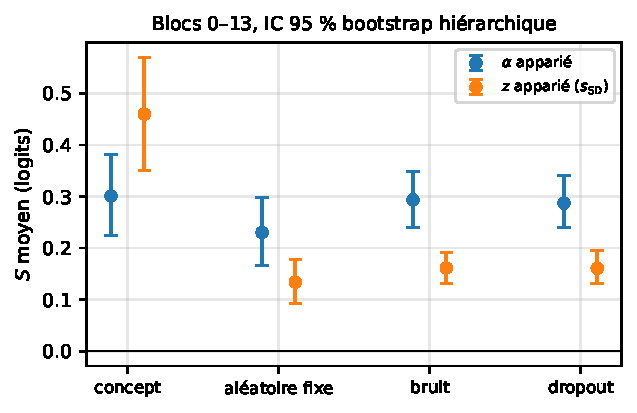
\includegraphics[width=\textwidth]{family_ordering.pdf}
\caption{Ordonnancement des familles sur la bande vive, avec intervalles bootstrap
hiérarchiques à \SI{95}{\percent}.}
\end{figure}

\subsection{Le basculement d'ordre des étiquettes}

Même après appariement, la lettre imprimée en premier compte :

\begin{center}
\begin{tabular}{lrrr}
\toprule
\code{label\_order} & $S$ moyen & part $S>0$ & $n$ \\
\midrule
AB (la première phrase est \og A \fg) & \num{0.379} & \num{0.657} & \num{33880} \\
BA (la première phrase est \og B \fg) & \num{0.160} & \num{0.565} & \num{33880} \\
\midrule
ordre de présentation 0 & \num{0.271} & --- & --- \\
ordre de présentation 1 & \num{0.268} & --- & --- \\
\bottomrule
\end{tabular}
\end{center}

\noindent
Un ré-étiquetage purement cosmétique --- mêmes phrases, même ordre physique, même
perturbation --- change la localisation mesurée d'un facteur \num{2.4}, alors que l'ordre
physique est parfaitement équilibré. L'effet est positif dans les deux cas, mais son
amplitude n'est pas une propriété stable du modèle.

\begin{center}\fbox{\parbox{0.92\textwidth}{
\textbf{Recommandation 2.} Rapporter tout chiffre principal par ordre d'étiquettes, ou
étendre le plan jusqu'à comprendre ce basculement. Une valeur unique moyennée masque un
facteur 2.
}}\end{center}

\subsection{Biais A/B sur les sham}

Les \num{20} conditions sham distinctes ont \emph{toutes} $\ell_A > \ell_B$.

\begin{center}
\begin{tabular}{lr}
\toprule
Contraste sham moyen & \num{1.725} logit \\
Écart-type & \num{0.579} \\
Étendue & \num{0.375} à \num{2.75} \\
Part préférant A & \SI{100}{\percent} \\
Moyenne sous \code{label\_order} AB & \num{1.9875} \\
Moyenne sous \code{label\_order} BA & \num{1.4625} \\
Taux d'invalides & \SI{0}{\percent} \\
\bottomrule
\end{tabular}
\end{center}

\noindent
Le biais survit à l'inversion des étiquettes : c'est une préférence pour la
\emph{lettre} A, pas pour la première position. Le contrôle \code{label\_order} a rempli
son office.

\paragraph{Défaut de comptage.} \code{trials.csv} contient \num{40} lignes sham pour
\num{20} conditions distinctes, chacune dupliquée avec des logits identiques au bit près :
le raccord des deux \emph{jobs} a écrit un bloc sham par \emph{job}. C'est sans effet sur
l'indicateur ajusté (la passe avant est déterministe, la même valeur est soustraite), mais
\code{summary.json} annonce \code{sham.n\_trials: 40} pour \num{20} mesures. À corriger
avant toute citation.

\subsection{Taux de réponses invalides}

\begin{center}
\begin{tabular}{lrr}
\toprule
Famille & Taux d'invalides & Taux d'égalités \\
\midrule
concept          & \num{0.0199} & \num{0.324} \\
aléatoire fixe   & \num{0.0037} & \num{0.456} \\
\emph{dropout}   & \num{0.0008} & \num{0.481} \\
bruit            & \num{0.0001} & \num{0.459} \\
\midrule
\textbf{global}  & \num{0.0083} & \num{0.414} \\
\bottomrule
\end{tabular}
\end{center}

\noindent
Aucune valeur non finie. Le taux d'invalides est négligeable jusqu'à $\alpha = 8$ puis
croît avec la dose : \num{0.0071} à $\alpha=16$, \num{0.0101} à $32$, \num{0.0289} à
$64$, \num{0.0539} à $128$. Il est concentré sur la famille conceptuelle, qui est la
seule à atteindre les amplitudes physiques extrêmes sous appariement en $z$
(section~\ref{sec:zmad}).

\subsection{Amplitude réalisée par token et taux \texorpdfstring{$p$}{p}}

Pour les familles additives, l'amplitude réalisée reproduit la demande à \num{5e-5} près.
Le \emph{dropout} est le seul cas où la dose demandée n'est pas atteinte :

\begin{center}
\begin{tabular}{rrrr}
\toprule
$\alpha$ demandé & $\alpha$ réalisé (\emph{dropout}) & $p$ moyen & $p$ maximal \\
\midrule
8   & \num{7.90}  & \num{0.396} & \num{0.985} \\
16  & \num{15.55} & \num{0.607} & \num{0.996} \\
32  & \num{29.95} & \num{0.797} & \num{0.999} \\
64  & \num{55.92} & \num{0.922} & \num{0.9998} \\
128 & \num{99.44} & \num{0.976} & \num{0.99994} \\
\bottomrule
\end{tabular}
\end{center}

\noindent
\textbf{L'axe de dose du \emph{dropout} est dégénéré en haut de grille.} Le taux ne peut
pas dépasser 1 ; les trois ou quatre doses supérieures correspondent toutes à
\og phrase oblitérée \fg{} et ne sont donc pas des augmentations de dose. La chute du
\emph{dropout} de \num{0.81} à $\alpha=16$ vers \num{0.52} à $\alpha=128$ est ce plafond,
pas une relation dose--réponse.

\subsection{Seuils \texorpdfstring{$\alpha_{75}$}{alpha75} et \texorpdfstring{$z_{75}$}{z75}}

Sur \num{508} courbes ajustées, \textbf{17 seuils seulement sont rapportables} au sens de
la section 5.10 (transition encadrée \emph{et} seuil intérieur à la plage testée) :

\begin{center}
\begin{tabular}{lrr}
\toprule
Indicateur / appariement & Courbes & Seuils rapportables \\
\midrule
ajusté / $z$      & 127 & 15 \\
ajusté / $\alpha$ & 127 & 2 \\
brut / $z$        & 127 & 0 \\
brut / $\alpha$   & 127 & 0 \\
\bottomrule
\end{tabular}
\end{center}

\noindent
La cause n'est pas le bruit, c'est la \emph{forme}. Sous appariement en $\alpha$, les
\num{14} couches vives des familles aléatoire, bruit et \emph{dropout} culminent
\emph{avant} la dose maximale puis redescendent, perdant \num{0.16} à \num{0.21}
d'\emph{accuracy}, alors que \code{fit\_psychometric} ajuste une logistique monotone.

\begin{center}
\begin{tabular}{lrr}
\toprule
Famille & Chute pic$\to$dose max ($\alpha$) & Chute pic$\to$dose max ($z$) \\
\midrule
concept          & \num{0.049} & \num{0.022} \\
\emph{dropout}   & \num{0.156} & \num{0.096} \\
bruit            & \num{0.175} & \num{0.092} \\
aléatoire fixe   & \num{0.206} & \num{0.079} \\
\bottomrule
\end{tabular}
\end{center}

\noindent
Le concept est nettement plus monotone que les témoins : il \emph{sature}, les témoins
\emph{s'inversent} activement. C'est une signature spécifique au concept, indépendante de
l'échelle.

\begin{center}\fbox{\parbox{0.92\textwidth}{
\textbf{Recommandation 3.} Ne citer aucun seuil à \SI{75}{\percent} issu de ce balayage,
ou remplacer la logistique monotone par un modèle admettant une réponse non monotone. La
section 5.10 prévoit explicitement ce cas de figure et interdit l'annonce d'un seuil.
}}\end{center}

\subsection{Interaction famille \texorpdfstring{$\times$}{x} couche \texorpdfstring{$\times$}{x} dose}

\begin{figure}[h]
\centering
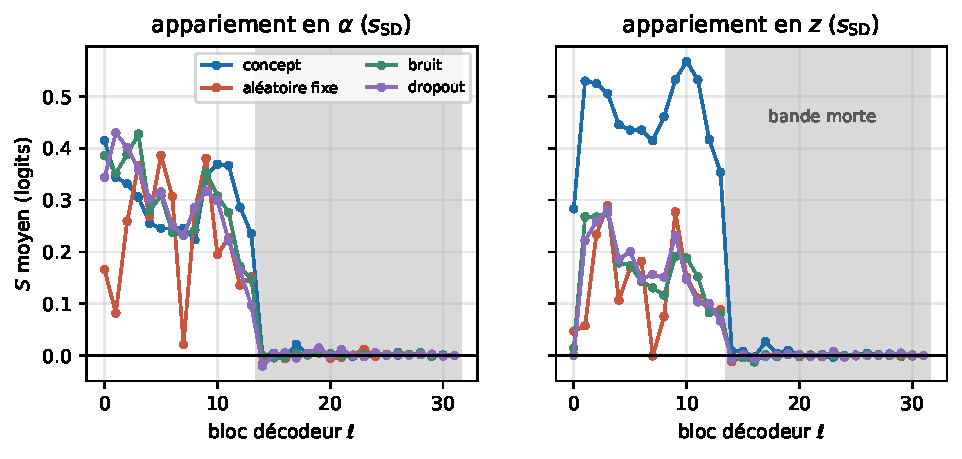
\includegraphics[width=\textwidth]{depth_profile.pdf}
\caption{Profil de profondeur de $S$. La bande grisée marque les blocs 14--31, où la
mesure est exactement au hasard. Le contraste entre les deux panneaux est l'objet de la
section~\ref{sec:zmad}.}
\end{figure}

\begin{table}[h]
\centering
\caption{$S$ moyen par bloc et par famille, appariements confondus. La coupure au bloc 14
est nette : le concept passe de \num{0.300} à \num{0.005} en un bloc.}
\label{tab:depth}
\begin{tabular}{rrrrrrr}
\toprule
Bloc & concept & aléatoire & bruit & \emph{dropout} & \emph{acc.} ajustée & taux d'égalités \\
\midrule
0  & \num{0.343} & \num{0.101} & \num{0.183} & \num{0.157} & \num{0.578} & \num{0.252} \\
1  & \num{0.445} & \num{0.069} & \num{0.306} & \num{0.316} & \num{0.628} & \num{0.149} \\
2  & \num{0.437} & \num{0.245} & \num{0.322} & \num{0.324} & \num{0.659} & \num{0.158} \\
3  & \num{0.415} & \num{0.324} & \num{0.345} & \num{0.317} & \num{0.656} & \num{0.150} \\
4  & \num{0.359} & \num{0.180} & \num{0.225} & \num{0.239} & \num{0.612} & \num{0.190} \\
5  & \num{0.349} & \num{0.268} & \num{0.235} & \num{0.253} & \num{0.627} & \num{0.197} \\
6  & \num{0.349} & \num{0.239} & \num{0.186} & \num{0.195} & \num{0.599} & \num{0.194} \\
7  & \num{0.338} & \num{0.009} & \num{0.177} & \num{0.191} & \num{0.556} & \num{0.174} \\
8  & \num{0.353} & \num{0.168} & \num{0.173} & \num{0.212} & \num{0.590} & \num{0.200} \\
9  & \num{0.448} & \num{0.324} & \num{0.265} & \num{0.270} & \num{0.666} & \num{0.195} \\
10 & \num{0.478} & \num{0.171} & \num{0.243} & \num{0.216} & \num{0.621} & \num{0.203} \\
11 & \num{0.457} & \num{0.164} & \num{0.208} & \num{0.157} & \num{0.639} & \num{0.225} \\
12 & \num{0.358} & \num{0.110} & \num{0.124} & \num{0.129} & \num{0.589} & \num{0.242} \\
13 & \num{0.300} & \num{0.118} & \num{0.111} & \num{0.080} & \num{0.620} & \num{0.276} \\
\midrule
14 & \num{0.005} & \num{-0.014} & \num{-0.004} & \num{-0.013} & \num{0.488} & \num{0.385} \\
20 & \num{0.002} & \num{-0.004} & \num{0.001}  & \num{0.001}  & \num{0.491} & \num{0.556} \\
30 & \num{0.001} & \num{0.001}  & \num{0.000}  & \num{-0.001} & \num{0.502} & \num{0.801} \\
31 & ---         & \num{0.000}  & \num{0.000}  & \num{0.000}  & \num{0.500} & \num{1.000} \\
\bottomrule
\end{tabular}
\end{table}

\noindent
\textbf{La coupure n'est pas la perturbation qui s'estompe.} La magnitude du contraste
ajusté décroît \emph{continûment} avec la profondeur --- \num{1.60} au bloc 0, \num{0.86}
au bloc 13, \num{0.52} au bloc 14, \num{0.06} au bloc 30 --- alors que l'\emph{accuracy}
passe de \num{0.77} à \num{0.50} en un seul bloc. La perturbation atteint encore le bloc
14 avec la moitié de la magnitude qu'elle avait au bloc 13 ; ce qui disparaît est
l'\emph{information sur quelle phrase}, pas la magnitude.

\subsection{Bloc 31 : structurellement mort}
\label{sec:block31}

Le taux d'égalités vaut exactement \num{1.000} à toutes les doses, y compris à une
amplitude réalisée de \num{127}. Le \emph{hook} est posé sur la sortie du bloc décodeur
(\code{experiment1\_psychometrics.py:319}) ; la sortie du bloc 31 aux positions des
phrases n'est plus suivie que de la normalisation finale et de \code{lm\_head}, toutes
deux positionnelles. Elle ne peut jamais atteindre le token de réponse. La cellule
conceptuelle manquante au bloc 31 ne coûte donc rien.

\subsection{Mesures non disponibles}

La section 5.14 demande également $d'$, le critère et l'AUROC de la tâche de présence
appariée. Ces mesures relèvent de l'expérience 2, qui n'a pas été exécutée : elles sont
\textbf{sans objet pour ce balayage}.

\section{Validation du pipeline (section 5.11)}

Le critère est rempli \emph{sur les blocs 0--13 seulement}. Le contraste signé de la
famille conceptuelle est positif, son intervalle hiérarchique exclut zéro
($[\num{0.225};\ \num{0.381}]$ à $\alpha$ apparié), et les permutations d'ordre ne
renversent pas la conclusion (ordre physique : \num{0.271} contre \num{0.268}).

Deux réserves accompagnent cette validation.

\begin{enumerate}
\item Le basculement AB/BA d'un facteur \num{2.4} signifie que l'amplitude validée
      dépend d'un choix de présentation, même si son signe n'en dépend pas.
\item \textbf{La contamination rend la question 2AFC mal posée aux doses élevées.} Le
      diagnostic $P_{1\rightarrow2}$ sature à \num{0.65}--\num{1.47} en deux blocs et ne
      décroît jamais : plusieurs cellules dépassent \num{1.0}, ce qui signifie que la
      phrase \emph{non} ciblée porte plus de perturbation que de signal propre. La
      couverture est mince (blocs d'injection 0, 1 et 2, dose maximale uniquement, une
      seule paire), mais suffisante pour établir le fait. À $\alpha = 128$ la seconde
      phrase n'est pas un témoin : elle a été écrasée aussi. La localisation qui subsiste
      est le modèle suivant \emph{quelle phrase a été touchée en premier et le plus
      fort}, non un contraste propre entre un item perturbé et un item intact.
\end{enumerate}

\noindent
La contamination est par ailleurs structurellement unidirectionnelle : seul
\code{target\_index = 0} est sondé, et le sens inverse est exactement nul par
construction, l'attention étant causale. Les deux conditions de cible ne sont donc pas
symétriques, et aucun équilibrage d'essais ne le corrige.

\section{L'appariement en \texorpdfstring{$z$}{z} : \texorpdfstring{$\ssd$}{s\_SD} contre \texorpdfstring{$\smad$}{s\_MAD}}
\label{sec:zmad}

C'est la section principale de ce document. La section 5.10 prévoit la sensibilité MAD
comme une analyse secondaire. Les données montrent qu'elle corrige un défaut central.

\subsection{L'échelle SD est portée par un token par phrase}

L'expérience 0 estime $s(\ell,v)$ sur \num{616} positions issues de \num{100} phrases,
soit \num{6.16} tokens par phrase, sous \code{position\_policy = all\_sentence\_tokens}.
La distribution des projections est violemment asymétrique. Pour
\code{concept\_\_block\_05\_\_recursion} :

\begin{center}
\begin{tabular}{lrrrrr}
\toprule
médiane & p05 & p95 & moyenne & $\ssd$ & $\smad$ \\
\midrule
\num{-0.028} & \num{-525.8} & \num{0.160} & \num{-85.2} & \num{194.2} & \num{0.158} \\
\bottomrule
\end{tabular}
\end{center}

\noindent
Le \num{5}\textsuperscript{e} percentile vaut $-526$ tandis que le
\num{95}\textsuperscript{e} vaut $+0{,}16$. En modélisant la distribution comme une masse
au voisinage de la médiane plus une fraction $f$ à l'extrême, $f = |\text{moyenne} -
\text{médiane}| / |\text{extrême} - \text{médiane}|$ donne, sur la bande vive :

\begin{center}
\begin{tabular}{lrr}
\toprule
Famille & $f$ (médiane) & $f \times 6{,}16$ tokens/phrase \\
\midrule
concept          & \num{0.162} & \num{1.00} \\
aléatoire fixe   & \num{0.159} & \num{0.98} \\
bruit renouvelé  & \num{0.159} & \num{0.98} \\
\bottomrule
\end{tabular}
\end{center}

\noindent
\textbf{La même fraction, \num{0.159}, apparaît dans les trois familles, et
\num{0.159} $\times$ \num{6.16} $=$ \num{0.98}.} Exactement un token par phrase porte une
projection deux à trois ordres de grandeur au-dessus de tous les autres, quelle que soit
la direction --- conceptuelle ou aléatoire. Il s'agit du phénomène d'\emph{activation
massive} bien documenté chez Llama : un token par segment sert de puits d'attention et
porte une norme d'activation démesurée.

Conséquence directe : $\ssd(\ell,v)$ ne décrit pas la variabilité naturelle du token
\emph{typique} que la perturbation frappe. Elle décrit la position d'un unique
\emph{outlier}. Le cadrage définit $s(\ell,v)$ comme \og l'échelle de variabilité des
activations sans intervention projetées dans cette direction \fg ; sous SD, cette
définition est captée par un token qui n'est représentatif de rien.

\begin{figure}[h]
\centering
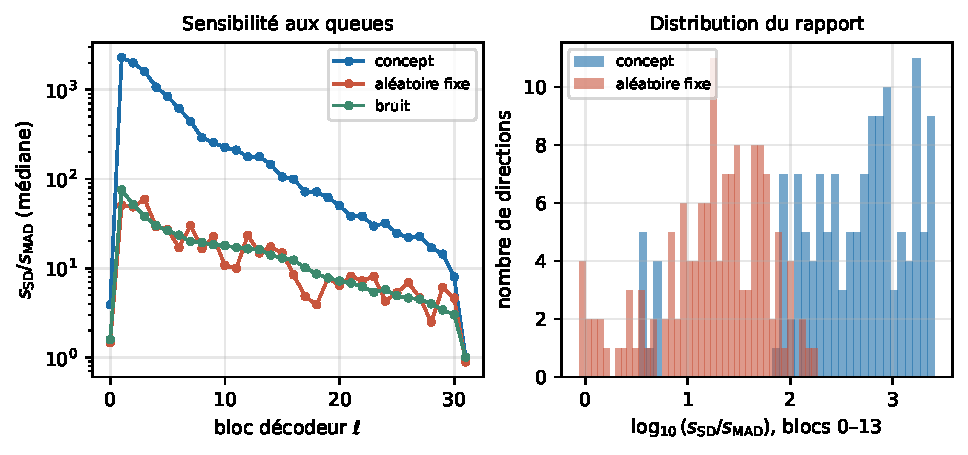
\includegraphics[width=\textwidth]{tail_ratio.pdf}
\caption{Rapport $\ssd/\smad$. À gauche, médiane par bloc et par famille (échelle
logarithmique). À droite, distribution du rapport sur la bande vive. Un rapport de 1
correspondrait à une distribution gaussienne : les valeurs observées vont jusqu'à
$10^3$. Les deux distributions sont presque disjointes. Le bloc 31 fait exception avec un
rapport de \num{0.96}--\num{1.00} pour les trois familles : la queue lourde y est absente,
ce qui recoupe le caractère structurellement particulier de ce bloc
(\S\ref{sec:block31}).}
\end{figure}

\begin{center}
\begin{tabular}{lrrr}
\toprule
Famille (blocs 0--13) & $\ssd$ médian & $\smad$ médian & $\ssd/\smad$ \\
\midrule
concept          & \num{98.8} & \num{0.219} & \num{506} \\
aléatoire fixe   & \num{1.83} & \num{0.097} & \num{20.1} \\
bruit renouvelé  & \num{1.94} & \num{0.097} & \num{21.2} \\
\bottomrule
\end{tabular}
\end{center}

\subsection{Ce que l'appariement en \texorpdfstring{$z$}{z} apparie réellement}

Le rapport d'échelle \emph{entre familles} est ce que la division par $s$ élimine. Il
diffère d'un facteur \num{20} selon l'estimateur retenu :

\begin{center}
\begin{tabular}{rrr|rrr}
\toprule
Bloc & $\ssd$ concept/aléat. & $\smad$ concept/aléat. &
Bloc & $\ssd$ concept/aléat. & $\smad$ concept/aléat. \\
\midrule
0 & \num{35.6}  & \num{13.4} & 7  & \num{30.9} & \num{2.09} \\
1 & \num{122.4} & \num{2.69} & 8  & \num{46.8} & \num{2.68} \\
2 & \num{89.0}  & \num{2.17} & 9  & \num{28.8} & \num{2.53} \\
3 & \num{50.1}  & \num{1.85} & 10 & \num{50.3} & \num{2.39} \\
4 & \num{63.0}  & \num{1.72} & 11 & \num{57.2} & \num{2.72} \\
5 & \num{56.3}  & \num{1.81} & 12 & \num{22.7} & \num{2.99} \\
6 & \num{67.3}  & \num{1.86} & 13 & \num{34.4} & \num{2.87} \\
\bottomrule
\end{tabular}
\end{center}

\noindent
Sous SD, une valeur de $z$ donnée achète au concept une amplitude physique \num{23} à
\num{122} fois supérieure à celle d'une direction aléatoire. Sous MAD, le facteur tombe
entre \num{1.7} et \num{3.0} sur les blocs 1--13 (le bloc 0, à \num{13.4}, fait
exception et se comporte à part sur presque toutes les mesures de ce balayage). En
amplitude réalisée, sur la bande vive :

\begin{center}
\begin{tabular}{lrrr}
\toprule
Famille & $\alpha$ médian ($z$ apparié, SD) & $\alpha$ maximal & $\alpha$ maximal ($\alpha$ apparié) \\
\midrule
concept          & \num{164}  & \num{3388} & 128 \\
aléatoire fixe   & \num{1.92} & \num{39.4} & 128 \\
bruit            & \num{1.94} & \num{39.8} & 128 \\
\emph{dropout}   & \num{1.94} & \num{39.8} & 128 \\
\bottomrule
\end{tabular}
\end{center}

\noindent
\noindent
Qu'une même valeur de $z$ livre des amplitudes physiques différentes n'est pas en soi un
défaut : c'est le principe de l'appariement standardisé, et la
section~\ref{sec:portee} y revient. Ce qui est en cause est l'\emph{ampleur} de l'écart.
Le balayage a poussé le concept jusqu'à $\alpha \approx 3400$, bien au-delà de tout ce que
la grille $\alpha$ explore, pendant que les témoins plafonnaient à $\alpha \approx 40$ ---
une région où leurs courbes commencent tout juste à monter. Aucune famille témoin n'est
donc testée près de sa transition. L'écart concept/témoins de \num{0.33} du
tableau~\ref{tab:S} sous appariement en $z$ mesure principalement cette différence
d'amplitude délivrée, et la section~\ref{sec:origine} montre que le facteur \num{56} à
\num{95} qui la produit est un artefact du contexte de calibration.

\subsection{Comparaison à amplitude physique appariée}

En regroupant les deux appariements et en liant par octaves d'amplitude réalisée, on
obtient la comparaison que le protocole cherchait :

\begin{figure}[h]
\centering
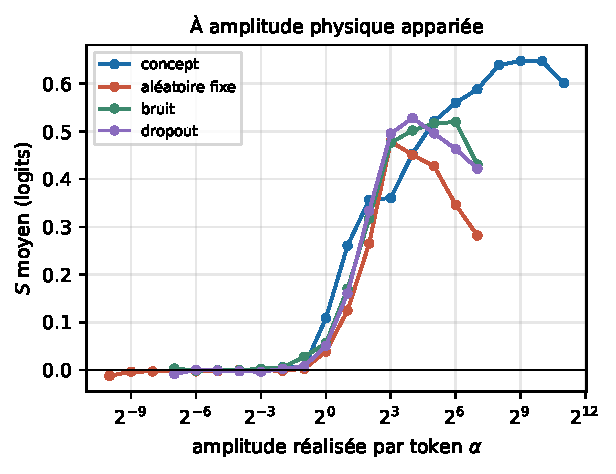
\includegraphics[width=0.62\textwidth]{matched_alpha.pdf}
\caption{$S$ en fonction de l'amplitude effectivement délivrée par token, bande vive,
appariements confondus. Le concept atteint seul les amplitudes supérieures à $2^{8}$.}
\end{figure}

\begin{center}
\begin{tabular}{lrrr}
\toprule
Paramétrisation & concept & témoins (min--max) & écart concept $-$ aléatoire \\
\midrule
$\alpha$ réalisé apparié (octaves communes) & \num{0.348} & \num{0.226}--\num{0.280} & $+\num{0.121}$ \\
$z_{\mathrm{MAD}}$ apparié (octaves communes) & \num{0.353} & \num{0.200}--\num{0.239} & $+\num{0.153}$ \\
$z_{\mathrm{SD}}$ apparié (octaves communes)  & \num{0.434} & \num{0.165}--\num{0.198} & $+\num{0.269}$ \\
\bottomrule
\end{tabular}
\end{center}

\noindent
L'ordonnancement \textbf{concept $>$ bruit $\approx$ \emph{dropout} $>$ aléatoire fixe}
est stable sous les trois paramétrisations : c'est le résultat robuste de ce balayage.
La figure~\ref{fig:sdmad} rend ce point visuellement : sous SD la courbe conceptuelle est
décalée de plusieurs octaves vers la gauche par rapport aux témoins, tandis que sous MAD
les quatre courbes se superposent presque, le concept conservant une avance d'environ une
octave.
Mais l'\emph{amplitude} de l'avantage conceptuel varie d'un facteur \num{2.2} selon la
paramétrisation, et la valeur SD est la plus extrême des trois. La standardisation MAD
se place entre les deux, beaucoup plus près de la comparaison à amplitude physique
appariée --- ce qui est exactement ce qu'on attend si la valeur SD était gonflée par
l'\emph{outlier}.

\begin{figure}[h]
\centering
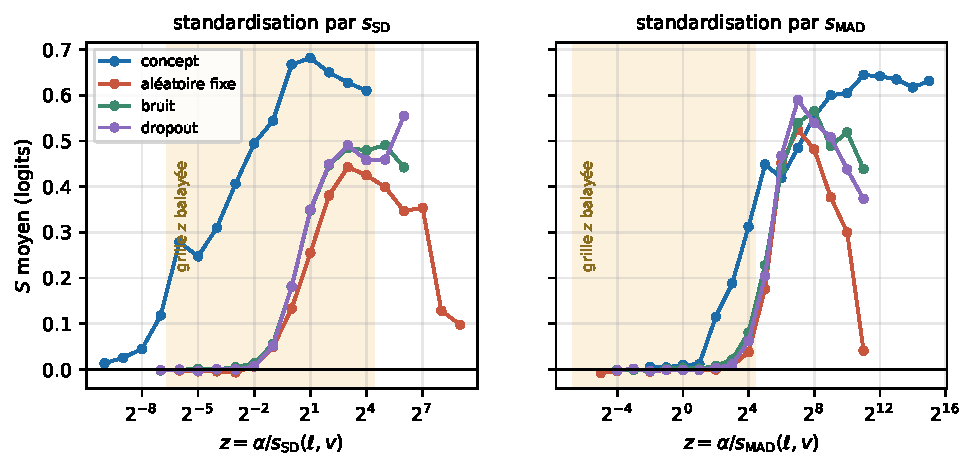
\includegraphics[width=\textwidth]{sd_vs_mad.pdf}
\caption{$S$ en fonction de $z$ sous les deux estimateurs, reconstruit à partir des
essais existants. La bande ambrée marque la grille $z \in [0{,}01;\,20{,}48]$
effectivement balayée. \textbf{Gauche (SD)} : cette grille place le concept sur son
plateau alors que les témoins n'ont pas encore décollé ; les courbes témoins plates
\emph{à l'intérieur de la fenêtre balayée} sont donc un artefact d'étendue de grille, et
la séparation apparente des familles est une séparation d'amplitude délivrée.
\textbf{Droite (MAD)} : les quatre courbes se superposent presque, le concept montant
environ une octave plus tôt ; la grille balayée y tombe presque entièrement sous le seuil
de toutes les familles, ce qui montre qu'une réexécution à grille inchangée ne
mesurerait rien.}
\label{fig:sdmad}
\end{figure}

\subsection{D'où vient le problème : contexte de calibration, non implémentation}
\label{sec:origine}

Trois causes étaient possibles : un défaut d'implémentation, un problème de données, ou
autre chose. La réponse est la troisième, elle est identifiable dans le code, et elle est
\emph{documentée dans la configuration elle-même}.

\paragraph{Ce n'est pas un défaut d'implémentation.} Les vérifications sont négatives.
L'écart-type est calculé correctement ; \code{direction\_bank.scale()} applique bien
l'échelle de la direction à la famille qui la porte ; la tokenisation utilise
\code{add\_special\_tokens=False}, donc aucun token BOS n'est ajouté par erreur ; et
\code{step\_01\_02\_collect\_natural\_activations.py} vérifie même l'absence de dérive de
tokenisation avant de collecter. Le code fait exactement ce qu'on lui demande.

\paragraph{Ce n'est pas non plus un problème de données.} Les \num{100} phrases de
\code{LOCALIZATION\_SENTENCES} sont les mêmes des deux côtés.

\paragraph{C'est le \emph{contexte de présentation} de la calibration.} Le fichier
\code{development\_full.yaml} rend chaque phrase \emph{seule} :

\begin{center}
\code{context\_id: isolated\_sentence\_development} \quad
\code{template: "\{sentence\}"} \quad
\code{position\_policy: all\_sentence\_tokens}
\end{center}

\noindent
Chaque phrase constitue donc sa propre séquence, et son premier token occupe la
\textbf{position 0}. C'est la position de puits d'attention, où Llama loge une activation
de norme démesurée --- le phénomène d'\emph{activation massive}. La politique
\code{all\_sentence\_tokens} l'inclut dans l'échantillon.

Dans l'expérience 1, les mêmes phrases sont enchâssées dans le prompt 2AFC complet
(gabarit de conversation, consigne, étiquettes \og A) \fg{} et \og B) \fg). Les tokens
perturbés y occupent les positions \num{40} à \num{80} environ, et
\code{build\_localization\_prompt} exclut même l'étiquette du \code{token\_range}.
\textbf{Aucun token perturbé n'est jamais en position 0.}

L'en-tête de la configuration annonce exactement cette limite :

\begin{quote}\small
\code{\# This is deliberately marked development: the isolated-sentence context must}\\
\code{\# be replaced by the exact behavioural prompt context before protocol freezing.}
\end{quote}

\noindent
Le drapeau \code{protocol\_status: development} et l'obligation de passer
\code{-{}-allow\_calibration\_mismatch} sont les garde-fous prévus pour ce cas. Ils ont
fonctionné : rien ici n'a été contourné silencieusement.

\subsection{Mesure directe des deux contextes}
\label{sec:probe}

L'inférence ci-dessus a été vérifiée par la mesure (\emph{job} \num{8174},
\code{results/experiment1/context\_probe/}). Les mêmes phrases et les mêmes directions
sont projetées dans les deux contextes : phrase isolée (ce que l'expérience 0 calibre) et
prompt 2AFC sur l'intervalle de tokens que l'expérience 1 perturbe réellement.

\begin{table}[h]
\centering
\caption{Échelles mesurées dans les deux contextes (médiane sur les directions de chaque
famille). \og queue \fg{} est la masse de queue $f$ définie plus haut.}
\label{tab:probe}
\begin{tabular}{rl|rrrr|rrrr}
\toprule
& & \multicolumn{4}{c|}{\textbf{phrase isolée} (calibration)}
  & \multicolumn{4}{c}{\textbf{prompt 2AFC} (perturbé)} \\
Bloc & Famille & $\ssd$ & $\smad$ & rapport & queue
               & $\ssd$ & $\smad$ & rapport & queue \\
\midrule
1  & concept   & \num{198.67} & \num{0.0800} & \num{2451} & \num{0.163}
               & \num{0.0248} & \num{0.0259} & \num{0.93} & \num{0.059} \\
1  & aléatoire & \num{3.55}   & \num{0.0249} & \num{141}  & \num{0.162}
               & \num{0.0203} & \num{0.0202} & \num{1.00} & \num{0.047} \\
5  & concept   & \num{184.21} & \num{0.1563} & \num{1196} & \num{0.163}
               & \num{0.1115} & \num{0.0885} & \num{1.11} & \num{0.067} \\
5  & aléatoire & \num{1.95}   & \num{0.0831} & \num{25.4} & \num{0.158}
               & \num{0.0562} & \num{0.0533} & \num{1.06} & \num{0.002} \\
9  & concept   & \num{160.82} & \num{0.2620} & \num{623}  & \num{0.163}
               & \num{0.1876} & \num{0.1904} & \num{0.98} & \num{0.019} \\
9  & aléatoire & \num{1.70}   & \num{0.1186} & \num{15.5} & \num{0.157}
               & \num{0.0824} & \num{0.0816} & \num{0.96} & \num{0.039} \\
13 & concept   & \num{146.98} & \num{0.3624} & \num{429}  & \num{0.163}
               & \num{0.2511} & \num{0.2454} & \num{0.91} & \num{0.042} \\
13 & aléatoire & \num{1.62}   & \num{0.1285} & \num{12.6} & \num{0.156}
               & \num{0.1069} & \num{0.1214} & \num{0.97} & \num{0.025} \\
\bottomrule
\end{tabular}
\end{table}

\noindent
Trois lectures, toutes décisives.

\begin{enumerate}
\item \textbf{Le token extrême est en position 0, et nulle part ailleurs.} Pour
      \code{recursion} au bloc 1, la projection maximale en valeur absolue vaut
      \textbf{\num{582.3}} en position 0 et \textbf{\num{0.399}} sur toutes les autres
      positions --- un facteur \num{1460}. La part de tokens en position 0 vaut
      \num{0.162} dans le contexte isolé, ce qui reproduit la masse de queue
      \num{0.159} estimée indépendamment sur la calibration. Dans le prompt, cette part
      vaut \textbf{exactement \num{0}}.
\item \textbf{La queue lourde disparaît entièrement dans le contexte comportemental.}
      $\ssd/\smad$ passe de \num{12.6}--\num{2451} à \textbf{\num{0.91}--\num{1.11}} pour
      toutes les familles. Dans le contexte que l'expérience 1 perturbe réellement, la
      distribution des projections est essentiellement gaussienne, et SD et MAD
      coïncident.
\item \textbf{Le rapport d'échelle entre familles s'effondre.} C'est la quantité que la
      division par $s$ élimine, et c'est elle qui distordait la comparaison :
\end{enumerate}

\begin{center}
\begin{tabular}{rrrrr}
\toprule
& \multicolumn{2}{c}{phrase isolée} & \multicolumn{2}{c}{prompt 2AFC} \\
Bloc & par $\ssd$ & par $\smad$ & par $\ssd$ & par $\smad$ \\
\midrule
1  & \num{55.9} & \num{3.21} & \num{1.22} & \num{1.28} \\
5  & \num{94.7} & \num{1.88} & \num{1.98} & \num{1.66} \\
9  & \num{94.4} & \num{2.21} & \num{2.28} & \num{2.33} \\
13 & \num{90.6} & \num{2.82} & \num{2.35} & \num{2.02} \\
\bottomrule
\end{tabular}
\end{center}

\noindent
Rapport d'échelle concept/aléatoire. Dans le bon contexte il vaut \num{1.2} à
\num{2.4}, et les deux estimateurs s'accordent. Le facteur \num{56}--\num{95} mesuré sur
la calibration est \emph{entièrement} l'effet du token de position 0.

\paragraph{Ce que cela change pour MAD.} Le rapprochement le plus parlant est que
$\smad$ mesuré dans le contexte isolé est proche de $\ssd$ mesuré dans le bon contexte
(bloc 13, concept : \num{0.362} contre \num{0.251} ; bloc 9 : \num{0.262} contre
\num{0.188}). \textbf{MAD approximait accidentellement la bonne quantité}, en jetant le
token qui n'aurait pas dû être dans l'échantillon. C'est pourquoi la réanalyse MAD de la
section précédente rapproche les résultats de la comparaison à amplitude physique
appariée : elle corrigeait le bon défaut, mais pour une raison indirecte.

Il s'ensuit que \textbf{MAD n'est pas le correctif}. Le correctif est de recalibrer dans
le contexte comportemental, ce que le protocole impose déjà avant gel. Une fois cela
fait, $\ssd \approx \smad$ et MAD redevient ce que la section 5.10 prévoit : un contrôle
de robustesse peu coûteux, et non une correction porteuse.

\paragraph{Ce que cela ne change pas : l'étendue de la grille.} La recalibration corrige
la distorsion \emph{entre} familles, pas l'étendue de la grille. Avec les échelles
mesurées dans le bon contexte, la grille $z$ actuelle livrerait encore :

\begin{center}
\begin{tabular}{rlrr}
\toprule
Bloc & Famille & $\alpha$ à $z=20{,}48$ & $z$ requis pour $\alpha=128$ \\
\midrule
1  & concept   & \num{0.51} & \num{5166} \\
5  & concept   & \num{2.28} & \num{1148} \\
9  & aléatoire & \num{1.69} & \num{1553} \\
13 & concept   & \num{5.14} & \num{510} \\
13 & aléatoire & \num{2.19} & \num{1198} \\
\bottomrule
\end{tabular}
\end{center}

\noindent
La dose maximale atteindrait $\alpha \approx 5$. Les deux défauts sont indépendants et
doivent être corrigés tous les deux.

\subsection{Statut des résultats en \texorpdfstring{$z$}{z} de ce balayage}
\label{sec:portee}

Il faut être explicite sur la portée. \textbf{L'appariement en $z$ n'a pas pour but de
donner la même amplitude physique à toutes les familles} --- c'est le rôle de
l'appariement en $\alpha$. Le cadrage définit deux paramétrisations précisément pour
qu'elles diffèrent, et H1c énonce que l'appariement en $z$ \emph{modifie} les écarts
observés à $\alpha$ apparié. Qu'une direction conceptuelle reçoive plus d'amplitude brute
à $z$ égal n'est donc pas en soi un défaut : c'est le mécanisme attendu.

Le défaut est que $s(\ell,v)$ a été estimée sur une distribution de tokens qui
\textbf{n'apparaît pas dans l'expérience}. Le $z$ du balayage \code{full32\_all} n'est pas
\og l'amplitude rapportée à la variabilité naturelle des activations perturbées \fg{} ;
c'est l'amplitude rapportée à la variabilité d'un échantillon dont \SI{16}{\percent} est
un token de puits d'attention que l'expérience 1 ne touche jamais.

En conséquence : \textbf{les courbes et écarts en $z$ de ce balayage ne doivent pas être
interprétés}, ni pour confirmer ni pour infirmer H1c. Les résultats en $\alpha$ ne sont
pas concernés --- ils ne font intervenir aucune échelle calibrée --- et restent la base
défendable de ce document, avec les réserves des sections précédentes.

\subsection{Réponse à la question posée : faut-il tester MAD ?}

\textbf{Oui, mais comme diagnostic et comme contrôle, pas comme correctif} --- et sans
relancer le balayage tel quel. Quatre points.

\paragraph{1. MAD n'est pas le correctif ; la recalibration l'est.} La
section~\ref{sec:probe} l'établit par la mesure : dans le contexte comportemental, la
queue lourde n'existe pas et $\ssd \approx \smad$ (rapport \num{0.91}--\num{1.11}). Le
défaut n'est donc pas l'estimateur mais l'échantillon sur lequel il est appliqué. Le
correctif est de recalibrer l'expérience 0 dans le contexte du prompt 2AFC, ce que
\code{development\_full.yaml} impose déjà avant gel. MAD reste utile pour deux raisons :
il a servi à \emph{détecter} le problème, et une fois la recalibration faite il redevient
le contrôle de robustesse peu coûteux que prévoit la section 5.10.

\paragraph{2. Réexécuter avec la même grille $z$ ne produirait rien.} Que l'on passe à
MAD ou que l'on recalibre dans le bon contexte, l'échelle obtenue est de 20 à 500 fois
plus petite que $\ssd$ mesurée sur phrases isolées. Sous MAD, la grille actuelle
livrerait :

\begin{center}
\begin{tabular}{lrrr}
\toprule
Famille & $\smad$ médian & $\alpha$ à $z=0{,}01$ & $\alpha$ à $z=20{,}48$ \\
\midrule
concept          & \num{0.220} & \num{0.0022} & \num{4.51} \\
aléatoire fixe   & \num{0.095} & \num{0.00095} & \num{1.95} \\
bruit            & \num{0.096} & \num{0.00096} & \num{1.97} \\
\emph{dropout}   & \num{0.096} & \num{0.00096} & \num{1.97} \\
\bottomrule
\end{tabular}
\end{center}

\noindent
La dose \emph{maximale} atteindrait $\alpha \approx 2$ pour les témoins, où $S \approx
0{,}16$ et la courbe commence à peine. Les quatre familles rendraient des courbes plates
ou à peine naissantes, et l'on conclurait à tort à une absence d'effet. \textbf{Pour
couvrir l'intervalle $\alpha \in [0{,}25;\,128]$ sous MAD, il faut $z$ de $\approx 1$ à
$\approx 1340$}, soit environ six octaves de plus que la grille actuelle.

\paragraph{3. La réanalyse MAD coûte zéro GPU.} $z = \alpha / s(\ell,v)$ est un
ré-étiquetage déterministe de l'axe de dose, par couche et par direction. Les essais à
$\alpha$ apparié contiennent donc déjà toutes les observations qu'un balayage en
$z_{\mathrm{MAD}}$ produirait : seuls les points de grille diffèrent. Les courbes
$z_{\mathrm{MAD}}$ de la figure ci-dessus et la ligne correspondante du tableau
précédent ont été obtenues ainsi, à partir des \num{306240} essais existants. Le
recouvrement en $z_{\mathrm{MAD}}$ entre familles couvre \num{12} octaves
($z \approx 0{,}5$ à $z \approx 2000$), soit autant que sous SD, et suffit largement à
comparer les familles.

\paragraph{4. La recalibration est peu coûteuse aussi.} L'expérience 0 ne fait que des
passes avant sans intervention. La sonde de la section~\ref{sec:probe} a mesuré les deux
contextes sur \num{100} phrases et \num{4} blocs en moins de dix minutes sur un seul GPU ;
les \num{32} blocs et les \num{20} directions de la calibration complète restent du même
ordre. Le coût n'est pas un argument pour conserver le contexte isolé.

\begin{center}\fbox{\parbox{0.92\textwidth}{
\textbf{Recommandation 4 (correctif principal).} Recalibrer l'expérience 0 dans le
contexte comportemental : remplacer \code{template: "\{sentence\}"} par le prompt 2AFC
rendu, et restreindre \code{position\_policy} aux tokens que l'expérience 1 perturbe
effectivement, c'est-à-dire l'intervalle que renvoie \code{build\_localization\_prompt}
sans l'étiquette. C'est ce que l'en-tête de \code{development\_full.yaml} exige déjà avant
gel, et c'est la condition pour que $z$ signifie ce que le cadrage dit qu'il signifie.

\medskip
\textbf{Recommandation 4bis (diagnostic, immédiat).} En attendant, produire l'analyse MAD
par \emph{réanalyse} du balayage existant : option \code{-{}-estimator mad} sur le chemin
d'analyse (\code{direction\_bank.py} expose déjà \code{ESTIMATOR\_FIELDS} et
\code{experiment1\_psychometrics.py} accepte déjà \code{-{}-estimator}), en reliant les
essais par leur \code{realized\_amplitude} plutôt que par la dose demandée. Zéro GPU.
}}\end{center}

\paragraph{Réserve sur la précision de MAD.} Le bootstrap par grappes de phrases de
l'expérience 0 donne un coefficient de variation médian de \num{0.008} pour $\ssd$ contre
\num{0.049} pour $\smad$. MAD est environ six fois plus bruité --- ce qui est attendu
pour un estimateur robuste --- mais reste précis à \SI{5}{\percent} près, largement
suffisant devant les écarts d'un facteur \num{20} à \num{500} dont il s'agit ici. Cette
réserve disparaît après recalibration : dans le contexte comportemental les deux
estimateurs coïncident, et SD, plus précis, redevient le choix primaire que le cadrage
lui donne.

\section{Anomalies}

\subsection{La famille \og concept \fg{} est un axe signé, et un concept en est le pôle négatif}

Sur la bande vive, les quatre concepts ne se comportent pas de la même manière :

\begin{center}
\begin{tabular}{lrr}
\toprule
Concept & $S$ ($\alpha$ apparié) & $S$ ($z$ apparié) \\
\midrule
Dust        & \num{0.111} & \num{0.109} \\
Satellites  & \num{0.330} & \num{0.486} \\
recursion   & \num{0.372} & \num{0.605} \\
shutdown    & \num{0.391} & \num{0.640} \\
\bottomrule
\end{tabular}
\end{center}

\noindent
Dust est inerte sous les \emph{deux} appariements, à amplitude réalisée identique : ce
n'est pas un artefact d'échelle, c'est la direction elle-même. Le chargement des vecteurs
sauvegardés l'explique. Sur les blocs 2--14, la première composante principale capte
\SI{63}{\percent} à \SI{86}{\percent} de la variance entre les quatre vecteurs
conceptuels. La structure de cet axe, mesurée directement sur les vecteurs
sauvegardés, est \emph{Dust contre (recursion, shutdown)} :

\begin{center}
\begin{tabular}{lr@{\qquad}lr}
\multicolumn{4}{c}{\textbf{Bloc 11 --- cosinus entre vecteurs conceptuels}} \\
\toprule
Dust $\cdot$ recursion  & \num{-0.742} & recursion $\cdot$ shutdown   & \num{+0.724} \\
Dust $\cdot$ shutdown   & \num{-0.603} & Satellites $\cdot$ recursion & \num{+0.259} \\
Dust $\cdot$ Satellites & \num{-0.331} & Satellites $\cdot$ shutdown  & \num{+0.216} \\
\midrule
\multicolumn{4}{l}{\emph{Chargements sur PC1 (blocs 2--14, orientés Dust négatif)}} \\
\multicolumn{4}{l}{\quad Dust \num{-0.83} \quad recursion \num{+0.42} \quad
 shutdown \num{+0.37} \quad Satellites \num{+0.03}} \\
\bottomrule
\end{tabular}
\end{center}

\noindent
Ce ne sont pas quatre sondes conceptuelles indépendantes. L'axe dominant oppose Dust
(chargement \num{-0.83}) à recursion et shutdown (\num{+0.42} et \num{+0.37}) ;
Satellites, avec un chargement de \num{0.03}, y est essentiellement \emph{orthogonal}.
Deux conclusions s'en dégagent, et elles ne sont pas identiques.

\begin{itemize}
\item \textbf{Le déficit de Dust s'aligne exactement sur le pôle négatif de PC1.} Le
      seul concept inerte est aussi le seul qui charge négativement, sur les 13 blocs
      vifs sans exception.
\item \textbf{Mais le succès des trois autres ne se réduit pas à leur chargement.}
      Satellites est quasi orthogonal à l'axe et obtient tout de même \num{0.486}, contre
      \num{0.605} et \num{0.640} pour les deux concepts fortement chargés. Un modèle
      \og une seule direction privilégiée \fg{} prédirait Satellites au niveau de Dust ;
      il ne l'est pas.
\end{itemize}

\noindent
La lecture défendable est donc intermédiaire : \og il existe une direction signée
privilégiée dont le pôle négatif ne localise pas, et un effet résiduel présent même hors
de cet axe \fg. Elle n'autorise ni \og le modèle introspecte des concepts \fg, ni sa
réfutation complète par la géométrie.

\paragraph{L'axe est identifié, et ce n'est pas un axe sémantique.} Une mesure
ultérieure (\code{code/analysis/probe\_sink\_alignment.py}, \emph{job} \num{8178})
tranche la question. Le cosinus absolu entre chaque direction et l'activation moyenne de
position 0 vaut :

\begin{center}
\begin{tabular}{rrrrrr}
\toprule
Bloc & Dust & Satellites & recursion & shutdown & les 3 aléatoires \\
\midrule
1  & \num{0.982} & \num{0.632} & \num{0.994} & \num{0.983} & \num{0.011}--\num{0.027} \\
5  & \num{0.928} & \num{0.340} & \num{0.958} & \num{0.894} & \num{0.005}--\num{0.011} \\
9  & \num{0.811} & \num{0.255} & \num{0.896} & \num{0.778} & \num{0.001}--\num{0.035} \\
13 & \num{0.744} & \num{0.205} & \num{0.856} & \num{0.699} & \num{0.007}--\num{0.011} \\
\bottomrule
\end{tabular}
\end{center}

\noindent
L'attendu isotrope en dimension \num{4096} est $1/\sqrt{4096} = \num{0.0156}$ : les
directions aléatoires tombent exactement dessus, les conceptuelles en sont \emph{quasi
colinéaires}. Les vecteurs conceptuels étant des \emph{moyennes} d'états cachés
(\code{concept\_vector\_type: avg}), ils héritent de la composante d'activation massive,
qui domine par sa norme (\num{547} en position 0 contre \num{1.7}--\num{9.7} ailleurs).

\textbf{PC1 est donc la direction de puits d'attention, non un axe sémantique.} Un
vecteur à $|\cos| = \num{0.99}$ ne conserve que \SI{14}{\percent} de sa norme dans un
sous-espace propre au concept. Les trois observations de cette section s'unifient :
Dust est le pôle négatif de cet axe, Satellites est le concept le \emph{moins} aligné
(\num{0.21}--\num{0.63}) et celui dont le chargement sur PC1 est quasi nul, et le rapport
d'échelle concept/aléatoire de la section~\ref{sec:zmad} s'en déduit
($\num{0.86}/\num{0.0156} \approx \num{55}$).

\begin{center}\fbox{\parbox{0.92\textwidth}{
\textbf{Recommandation 5 (révisée).} Retirer la composante de puits des vecteurs
\code{avg} avant de les utiliser comme directions d'injection, et vérifier ensuite que
PC1 cesse de capter \SI{61}{\percent}--\SI{83}{\percent} de la variance entre concepts.
Tant que ce n'est pas fait, l'écart concept/témoins ne peut pas être attribué au contenu
conceptuel.

\medskip
Le contrôle $-$Dust reste utile mais \textbf{change de sens} : il ne sépare \og axe
signé \fg{} de \og concept \fg{} que si l'axe est sémantique, ce qu'il n'est pas. Le
rejouer \emph{après} le retrait de la composante de puits.

\medskip
Ce chantier est \textbf{distinct de la recalibration} de la section~\ref{sec:origine} :
recalibrer corrige $s(\ell,v)$, pas ce que \emph{sont} les directions. Voir
\code{docs/livrables/calibration-contexte-probleme-et-correctif.md} \S4.
}}\end{center}

\subsection{Les directions aléatoires fixes s'anti-localisent aux blocs 7 et 12}

$S$ tombe à \num{0.009} au bloc 7 pour la famille aléatoire, contre \num{0.24} au bloc 6
et \num{0.17} au bloc 8. En détail, \code{fixed\_random\_\_block\_07\_\_0000} atteint une
\emph{accuracy} ajustée de \num{0.050} à $\alpha = 1$ \emph{et} à $\alpha = 2$
(\num{40} essais par cellule, soit $-5{,}7\sigma$ par cellule et $-8{,}1\sigma$ en
regroupant les deux doses) : \SI{95}{\percent} des essais déplacent les logits vers la
\emph{mauvaise} phrase.

Les \textbf{13} cellules significativement sous le hasard de tout le balayage
(\num{2794} cellules) appartiennent toutes à la famille aléatoire, toutes aux blocs 7 et
12, à doses moyennes, sous les deux appariements. Le concept, le bruit et le
\emph{dropout} ne s'inversent jamais ; et aux blocs 7 et 12 les \emph{trois} directions
aléatoires s'inversent, ce qui en fait une propriété de la profondeur et non d'un vecteur
malchanceux.

Mécanisme plausible : une poussée \emph{cohérente} (le même vecteur sur chaque token) à
ces profondeurs dégrade assez la phrase ciblée pour que le modèle nomme celle qu'il peut
encore lire. Le bruit renouvelé est incohérent entre tokens et ne le fait pas ; les
directions conceptuelles sont cohérentes mais ne le font pas non plus. Inexpliqué, et
mérite une sonde dédiée.

\subsection{Le bloc 16 est sous le hasard}

Hors égalités, le bloc 16 est à \num{0.466} ($-5{,}0\sigma$) et le bloc 14 à \num{0.479}
($-3{,}1\sigma$), alors que le bloc 17 est à \num{0.529} ($+4{,}0\sigma$). Sur 17 tests,
le bloc 16 survit à une correction pour comparaisons multiples. Faible en valeur absolue,
mais ce n'est pas du bruit.

\section{Lecture selon la grille de la section 5.15}

\begin{table}[h]
\centering
\caption{Confrontation des résultats à la grille d'interprétation du cadrage.}
\begin{tabular}{p{0.34\textwidth}p{0.60\textwidth}}
\toprule
Ligne de la grille 5.15 & Statut sur ce balayage \\
\midrule
Concept supérieur à $\alpha$ \emph{et} à $z$ appariés
& \textbf{Compatible, mais l'amplitude de l'avantage n'est pas établie.}
  L'ordonnancement tient sous les trois paramétrisations ; l'écart va de
  $+\num{0.121}$ à $+\num{0.269}$ selon l'échelle retenue. \\
\addlinespace
Avantage conceptuel à $\alpha$ mais pas à $z$
& \textbf{Écarté} : l'avantage est présent sous les deux, et plus grand sous $z_{SD}$. \\
\addlinespace
Familles comparables sous les deux appariements
& \textbf{Écarté} sur la bande vive ; \textbf{vérifié trivialement} sur les blocs 14--31,
  où toutes les familles sont à zéro. \\
\addlinespace
\emph{Dropout} détecté à plus faible amplitude que le bruit
& \textbf{Écarté} : bruit et \emph{dropout} sont indiscernables
  (\num{0.294} contre \num{0.287} à $\alpha$ apparié ; intervalles entièrement
  superposés). \\
\addlinespace
\emph{Dropout} et bruit indiscernables
& \textbf{Vérifié.} La détectabilité dépend de l'amplitude et du renouvellement par
  token, pas du caractère multiplicatif ou additif. \\
\addlinespace
Conclusion différente entre SD et MAD
& \textbf{Partiellement vérifié, et c'est le point sensible.} L'\emph{ordonnancement} est
  identique ; l'\emph{amplitude} de l'écart varie d'un facteur \num{2.2}. Conformément à
  la section 5.15, tout écart chiffré doit être présenté comme dépendant de la définition
  de l'échelle naturelle. \\
\bottomrule
\end{tabular}
\end{table}

\noindent
Une famille détectée à plus faible $\alpha$ produit un signal comportemental plus fort à
norme brute égale, sans que cela montre qu'elle soit plus détectable relativement à la
géométrie naturelle des activations. Sur ce balayage, la géométrie naturelle telle que
mesurée par SD est elle-même suspecte, ce qui rend la seconde lecture indisponible tant
que l'analyse MAD n'est pas produite.

\section{Synthèse des actions}

\begin{enumerate}
\item \textbf{Changer d'indicateur.} Rapporter \code{mean\_localization\_contrast} ($S$),
      déjà calculé, plutôt que \code{accuracy\_adjusted}, contaminé par le biais de
      lettre (\S\ref{sec:indicateur}).
\item \textbf{Recalibrer l'expérience 0 dans le contexte comportemental} --- le correctif
      principal. Remplacer le gabarit \code{"\{sentence\}"} par le prompt 2AFC rendu et
      restreindre les positions à celles que l'expérience 1 perturbe
      (\S\ref{sec:origine}, \S\ref{sec:probe}). L'en-tête de la configuration l'exige
      déjà avant gel.
\item \textbf{Ne pas interpréter les résultats en $z$} de ce balayage, dans aucun sens,
      tant que la recalibration n'est pas faite (\S\ref{sec:portee}).
\item \textbf{Produire l'analyse MAD par réanalyse} comme diagnostic immédiat, en
      reliant les essais par leur amplitude réalisée. Coût GPU nul (\S\ref{sec:zmad}).
\item \textbf{Étendre la grille $z$} avant toute nouvelle exécution : $z$ jusqu'à
      $\approx 1340$ sous MAD, $\approx 5000$ après recalibration au bloc 1. Ce défaut
      est \emph{indépendant} du précédent et survit à la recalibration.
\item \textbf{Documenter l'artefact d'étendue de grille} : les courbes témoins plates
      sous appariement en $z$ ne sont pas un résultat, elles sont l'effet d'une grille qui
      ne mène les témoins qu'à $\alpha \approx 40$.
\item \textbf{Injecter $-$Dust.} Une condition tranche entre \og axe signé \fg{} et
      \og concept \fg.
\item \textbf{Rapporter par ordre d'étiquettes}, ou expliquer le facteur \num{2.4}.
\item \textbf{Abandonner les seuils à \SI{75}{\percent}} issus de ce balayage, ou adopter
      un modèle non monotone.
\item \textbf{Plafonner la grille de \emph{dropout}} là où le taux sature
      ($\alpha \geq 32$ n'est plus une augmentation de dose).
\item \textbf{Augmenter \code{-{}-contamination\_trials}} pour couvrir les blocs 3--13 et
      plus d'une dose.
\item \textbf{Corriger \code{sham.n\_trials}} sur le résumé raccordé (\num{20} mesures,
      non \num{40}).
\end{enumerate}

\vspace{1em}
\noindent\rule{\textwidth}{0.4pt}\\
\footnotesize
Données : \code{results/experiment1/full32\_all} (\code{trials.csv}, \code{summary.json}),
\code{results/experiment\_0\_calibration/directional\_scales.csv}. Calibration
\code{development\_full.yaml}, statut \code{development} --- résultats hors protocole gelé.

\end{document}
